% !TeX TXS-program:bibliography = txs:///biber

\documentclass[
    paper=a4,
    fontsize=10pt,
    DIV=13,
    % twocolumn,
    oneside,
]{scrartcl}

%-------------------------------------------------------------------------------------------------
%   Packages, Style Guide
%-------------------------------------------------------------------------------------------------

%-------------------------------------------------------------------------------------------------
%   Packages
%-------------------------------------------------------------------------------------------------

\usepackage[utf8]{inputenc}                         % utf8 as input encoding
\usepackage[T1]{fontenc}                            % 8bit font encdoing
\usepackage[ngerman]{babel}                         % word seperation
\usepackage{microtype}                              % font expansion
\usepackage{libertine}                              % select font
\usepackage[libertine]{newtxmath}                   % select font for mathmode
\usepackage{scrlayer-scrpage}                       % Bessere Kopfzeilen

\usepackage[
    locale=DE,
    detect-all,
    per-mode=fraction,
]{siunitx}                                          % express SI units
\usepackage{amsmath}
\usepackage{booktabs}                               % better tables
\usepackage{tabularx}                               % tables with pagewidth
\usepackage{graphicx}                               % input pictures
\usepackage{svg}
\usepackage{xcolor}
\usepackage{flushend}
\usepackage{listingsutf8}

\usepackage{csquotes}                               % quote environment
\usepackage[
    backend=biber,
    style=ieee,
]{biblatex}                                          % source control

\usepackage{hyperref}                               % add hyperlinks

%-------------------------------------------------------------------------------------------------
%   Colors
%-------------------------------------------------------------------------------------------------

% \definecolor{colorblue}{HTML}{0480CC}				% color for weblinks
% \definecolor{colordarkblue}{HTML}{4C1DCC}			% no use case at the moment
% \definecolor{colorgreen}{HTML}{26CC1B}				% color for citations
% \definecolor{colorred}{HTML}{CC1204}				% color for pdf links
\definecolor{coloryellow}{HTML}{F0B707}			    % color for warnings

%-------------------------------------------------------------------------------------------------
%   Lengths
%-------------------------------------------------------------------------------------------------

\newlength{\imagewidth}
\setlength{\imagewidth}{0.7\columnwidth}

%-------------------------------------------------------------------------------------------------
%   Style Options
%-------------------------------------------------------------------------------------------------

\KOMAoptions{
    toc     =   listof,                                     % add table of figures in 
    % headsepline=true,                               % switch header rule
    numbers =   noendperiod,
}

\hypersetup{
    colorlinks=true,
    bookmarksnumbered=true,
}

\chead{Laborbericht Regelungstechnik}
\ohead{Versuch Nr. \printlabor}
\ihead{Jan Hoegen}

\flushbottom                                        % fill pages to bottom

\addbibresource{quellen.bib}

%-------------------------------------------------------------------------------------------------
%   Macros
%-------------------------------------------------------------------------------------------------
        
\newcommand{\missing}{%
    \textcolor{coloryellow}{MISSING}%
    \PackageWarning{rtl_labor}{You used the 'missing' macro at this line. Remove it before finalising document}%
}
\newcommand{\improve}{%
    \textcolor{coloryellow}{IMPROVE}%
    \PackageWarning{rtl_labor}{You used the 'improve' macro at this line. Remove it before finalising document}%
}

\newcommand{\legend}[1]{\par\footnotesize\textbf{Legende}: #1\par}
\newcommand{\figsource}[1]{\par\footnotesize\textbf{Quelle:} #1\par}

%-------------------------------------------------------------------------------------------------
%   Title Page
%-------------------------------------------------------------------------------------------------

\titlehead{%
    Hochschule Karlsruhe\\
    University of Applied Sciences\\
    Fakultät für Elektro- und Informationstechnik
}
\title{Laborbericht Regelungstechnik}

\publishers{Betreuer: Prof. Dr. Keller}

\author{%
    Jan Hoegen\thanks{%
        Matrikel-Nr. 82358. E-Mail \href{jan.hoegen@web,de}{jan.hoegen@web,de}}%
    % \and%
    % Rithik Kurmar\thanks{%
    %     Matrikel-Nr. . E-mail \href{}{}}
}

\newcommand{\labor}[1]{\newcommand{\printlabor}{#1}}

\AtBeginDocument{
    \subtitle{Versuch Nr.~\printlabor}
    
    \hypersetup{
        pdftitle = {RT Labor \printlabor\ | Hoegen},
    }
}

%-------------------------------------------------------------------------------------------------
%   Listing Settings
%-------------------------------------------------------------------------------------------------

\lstset{%
	frame			=	tb ,							%	horizontale Linie oben&unten
	breaklines		=	true,							%	Zeilenumbruch
	rulecolor		=	\color{black} ,					%	Rahmenfarbe ist schwarz
	% keywordstyle	=	\keywordcolor ,
	% commentstyle	=	\commentcolor ,
	% stringstyle		=	\stringcolor ,
	title			=	\lstname ,						%	Titel ist gleich dem Dateinamen
	basicstyle		=	\footnotesize\ttfamily ,		%	Kleine Schrift und Monospace
	% numbers			=	right,							%	Zeilennumber rechts (da marginalie links)
	inputencoding	=	utf8,  							% Input encoding
    extendedchars	=	true,  							% Extended ASCII
}
% \lstdefinestyle{TeX}{language=TeX,						%	Mehr Keywörter für TeX
%     morekeywords={vspcae, hspace, rule, ifdefined, newcommand, setlength, newlentgh, RequirePackage, ProvidesPackage, NeedsTexFormat, DeclareOption, ProcessOption}, 
% }
\lstset{literate=							%	ermöglicht Unicode-Zeichen in Listing!
  {á}{{\'a}}1 {é}{{\'e}}1 {í}{{\'i}}1 {ó}{{\'o}}1 {ú}{{\'u}}1
  {Á}{{\'A}}1 {É}{{\'E}}1 {Í}{{\'I}}1 {Ó}{{\'O}}1 {Ú}{{\'U}}1
  {à}{{\`a}}1 {è}{{\`e}}1 {ì}{{\`i}}1 {ò}{{\`o}}1 {ù}{{\`u}}1
  {À}{{\`A}}1 {È}{{\'E}}1 {Ì}{{\`I}}1 {Ò}{{\`O}}1 {Ù}{{\`U}}1
  {ä}{{\"a}}1 {ë}{{\"e}}1 {ï}{{\"i}}1 {ö}{{\"o}}1 {ü}{{\"u}}1
  {Ä}{{\"A}}1 {Ë}{{\"E}}1 {Ï}{{\"I}}1 {Ö}{{\"O}}1 {Ü}{{\"U}}1
  {â}{{\^a}}1 {ê}{{\^e}}1 {î}{{\^i}}1 {ô}{{\^o}}1 {û}{{\^u}}1
  {Â}{{\^A}}1 {Ê}{{\^E}}1 {Î}{{\^I}}1 {Ô}{{\^O}}1 {Û}{{\^U}}1
  {ã}{{\~a}}1 {?}{{\~e}}1 {i}{{\~i}}1 {õ}{{\~o}}1 {u}{{\~u}}1
  {Ã}{{\~A}}1 {?}{{\~E}}1 {I}{{\~I}}1 {Õ}{{\~O}}1 {U}{{\~U}}1
  {œ}{{\oe}}1 {Œ}{{\OE}}1 {æ}{{\ae}}1 {Æ}{{\AE}}1 {ß}{{\ss}}1
  {u}{{\H{u}}}1 {U}{{\H{U}}}1 {o}{{\H{o}}}1 {O}{{\H{O}}}1
  {ç}{{\c c}}1 {Ç}{{\c C}}1 {ø}{{\o}}1 {å}{{\r a}}1 {Å}{{\r A}}1
  {€}{{\euro}}1 {£}{{\pounds}}1 {«}{{\guillemotleft}}1
  {»}{{\guillemotright}}1 {ñ}{{\~n}}1 {Ñ}{{\~N}}1 {¿}{{?`}}1 {¡}{{!`}}1 
  {~}{{\textasciitilde}}1 {*}{{\normalfont{*}}}1
}

%-------------------------------------------------------------------------------------------------
%   Title Page
%-------------------------------------------------------------------------------------------------

\labor{1}
\date{\today}

%-------------------------------------------------------------------------------------------------
%   Begin
%-------------------------------------------------------------------------------------------------

\begin{document}

\maketitle

%-------------------------------------------------------------------------------------------------
%   Abstract
%-------------------------------------------------------------------------------------------------

% \begin{abstract}
%     \noindent    
%     \subsubsection*{Abstract}
%     \blindtext
% \end{abstract}

%-------------------------------------------------------------------------------------------------
%   Text
%-------------------------------------------------------------------------------------------------

\section{Darstellung von Sinussignalen}
    Die Funktionen aus der Versuchsanleitung \cite{versuch1} werden mit MATLAB simuliert und in Abbildung \ref{fig:sinus} dargestellt.

    \begin{align}
        x_1(t) &= 2 \cdot sin(2\pi \cdot \SI{2}{\kilo\hertz} \cdot t)\\
        x_1(t) &= 2 \cdot sin(2\pi \cdot \SI{6}{\kilo\hertz} \cdot t - \frac{\pi}{4})
    \end{align}

    Darüber hinaus wird das zusammen gesetzte Signal \(x_3(t)=x_1(t) \cdot x_1(t)\) sowie eine Lissajous-Figur mit \(x_1(t)\) auf der x-Achse und \(x_2(t)\) auf der y-Achse abgebildet. Es ist zu erkennen, dass die Frequenz das doppelte von \(x_1(t)\) mit einem DC-Offset beträgt. Der Code zum Erstellen der Grafiken ist in Anhang \ref{lst:sinus} zu sehen.

    \begin{figure}[hbt]
        \centering
        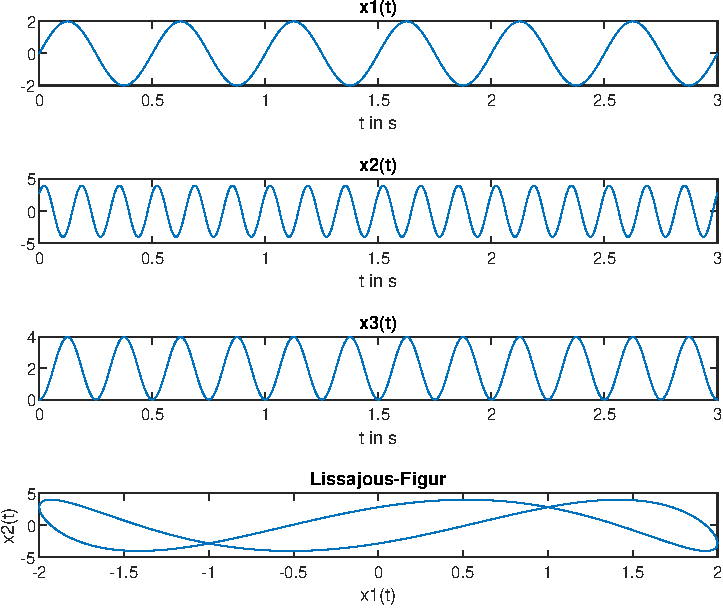
\includegraphics[width=\imagewidth]{../versuch1/sinus.pdf}
        \caption{Darstellung der Sinussignale}
        \legend{Darstellung mit \(10^3\) Abtastpunkten}
        \label{fig:sinus}
    \end{figure}

    \subsection{Fehlerhafte Darstellungen der Lissajous-Figur}
        Wird der Zeitbereich auf \SIrange{0}{3}{\second} gelegt und somit die Größenordnung um \(10^3\) erhöht, ist die Figur zur Abbildung \ref{fig:sinus} gleich. Wird der Zeitbereich auf leicht verschoben, entsteht ein nicht interpretierbares Bild. Diese Effekte sind durch den Aliasing-Effekt zu begründen.
        Beide Änderungen sind in Abbildung \ref{fig:lissajous} gezeigt.

        \begin{figure}[hbt]
            \centering
            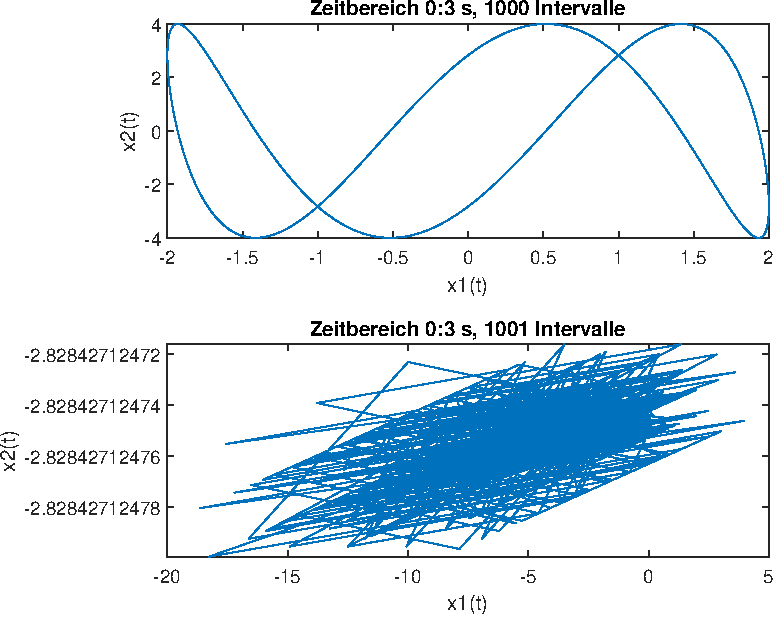
\includegraphics[width=\imagewidth]{../versuch1/lissjaou.pdf}
            \caption{Fehlerhafte Lissajous-Figuren}
            \label{fig:lissajous}
        \end{figure}

\section{Tiefpassanalyse}
    Für einen Tiefpass erster Ordnung gilt:
    \begin{align}
        \label{eq:tp}
        \frac{U_a}{U_e} = \frac{1}{1+jwRC}
    \end{align}

    Die Bauteilwerte mit einer Grenzfrequenz von \SI{100}{\kilo\hertz} und einem gewählten Kondensator \(C\) von \SI{1e-9}{\farad} berechnen sich zu:
    \begin{align}
        f_g &= \frac{1}{2 \pi RC} \overset{!}{=} \SI{1e5}{\hertz}\\
        \Rightarrow R&= \frac{1}{2 \pi \cdot f_g \cdot C }= \SI{1591.55}{\ohm}
    \end{align}

    Das Bodediagramm ist in Abbildung \ref{fig:bode} und die zugehörige Ortskurve in Abbildung \ref{fig:ortskurve} dargestellt. Da die Ortskurve achsensymmetrisch zur x-Achse ist, kann das Diagramm ohne den Verlust von Informationen um genau diese Spiegelung verkürzt werden. In MATLAB wird dies durch die Option \verb|ShowFullContour='off'| des \verb|nyquistplot|-Befehls erreicht. Der Code zum Erstellen der Diagramme findet sich in Anhang \ref{lst:tiefpass}.

    \begin{figure}
        \centering
        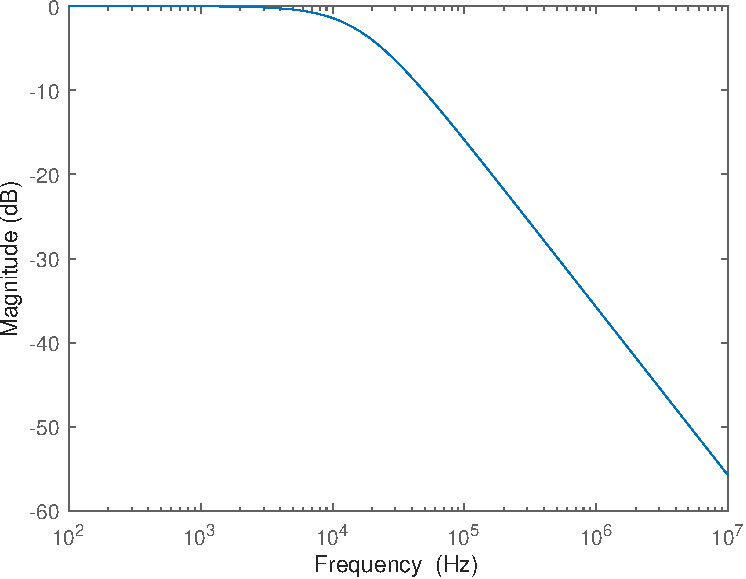
\includegraphics[width=\imagewidth]{../versuch1/bode.pdf}
        \caption{Bodediagramm des Tiefpasses}
        \label{fig:bode}
    \end{figure}

    \begin{figure}
        \centering
        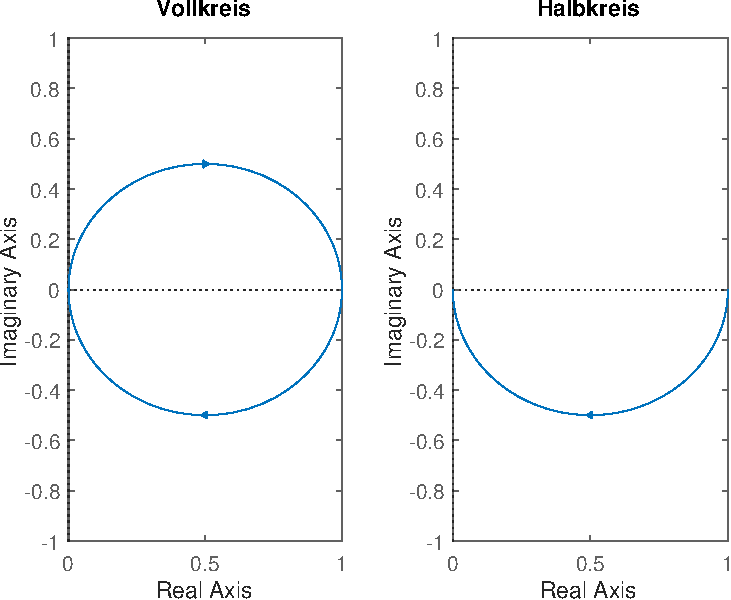
\includegraphics[width=\imagewidth]{../versuch1/ortskurve.pdf}
        \caption{Ortskurven des Tiefpasses}
        \label{fig:ortskurve}
    \end{figure}

\section{Temperaturregler}
    Nun wird ein Temperaturregler in Abbildung \ref{_schaltbild} simuliert. Der Zeitverlauf der eingestellten Solltemperatur, der Stellgröße und der Ausgangsgröße sind in Abbildung \ref{fig:temp_regler} dargestellt. Es ist zu erkennen, dass bei eingeschalteten Heizelement die Temperatur im Backofen schnell steigt bis zur Zieltemperatur von \SI{160}{\celsius}. Anschließend wird periodisch auf- und abgewärmt, bis die Führungsgröße auf \SI{0}{\celsius} verändert wird und die Temperatur absinkt. Die Parameter wurden im Anhang \ref{lst:temp_regler} definiert.

    \begin{figure}
        \centering
        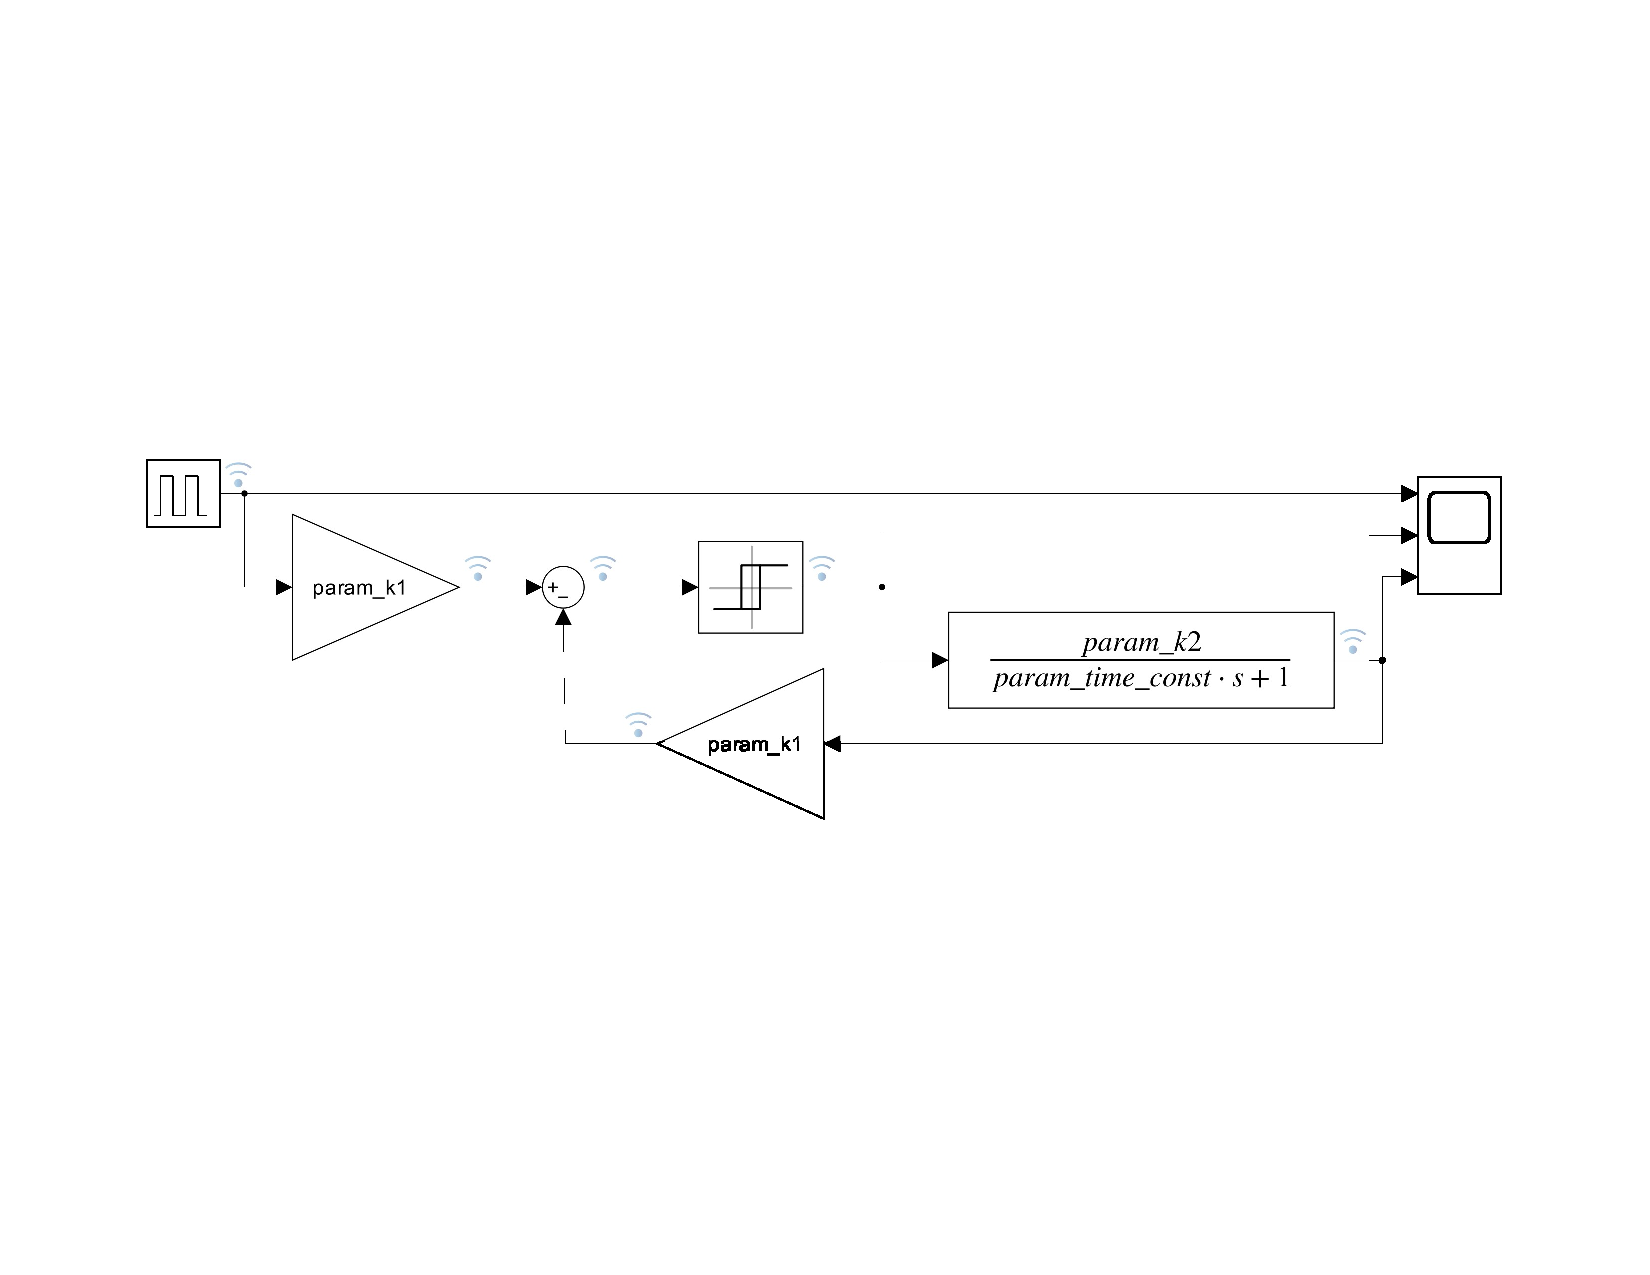
\includegraphics[width=1\imagewidth]{../versuch1/temp_regler_schaltbild.pdf}
        \caption{Blockschaltbild des Temperaturreglers}
        \label{fig:temp_regler_schaltbild}
    \end{figure}    

    \begin{figure*}
        \centering
        % 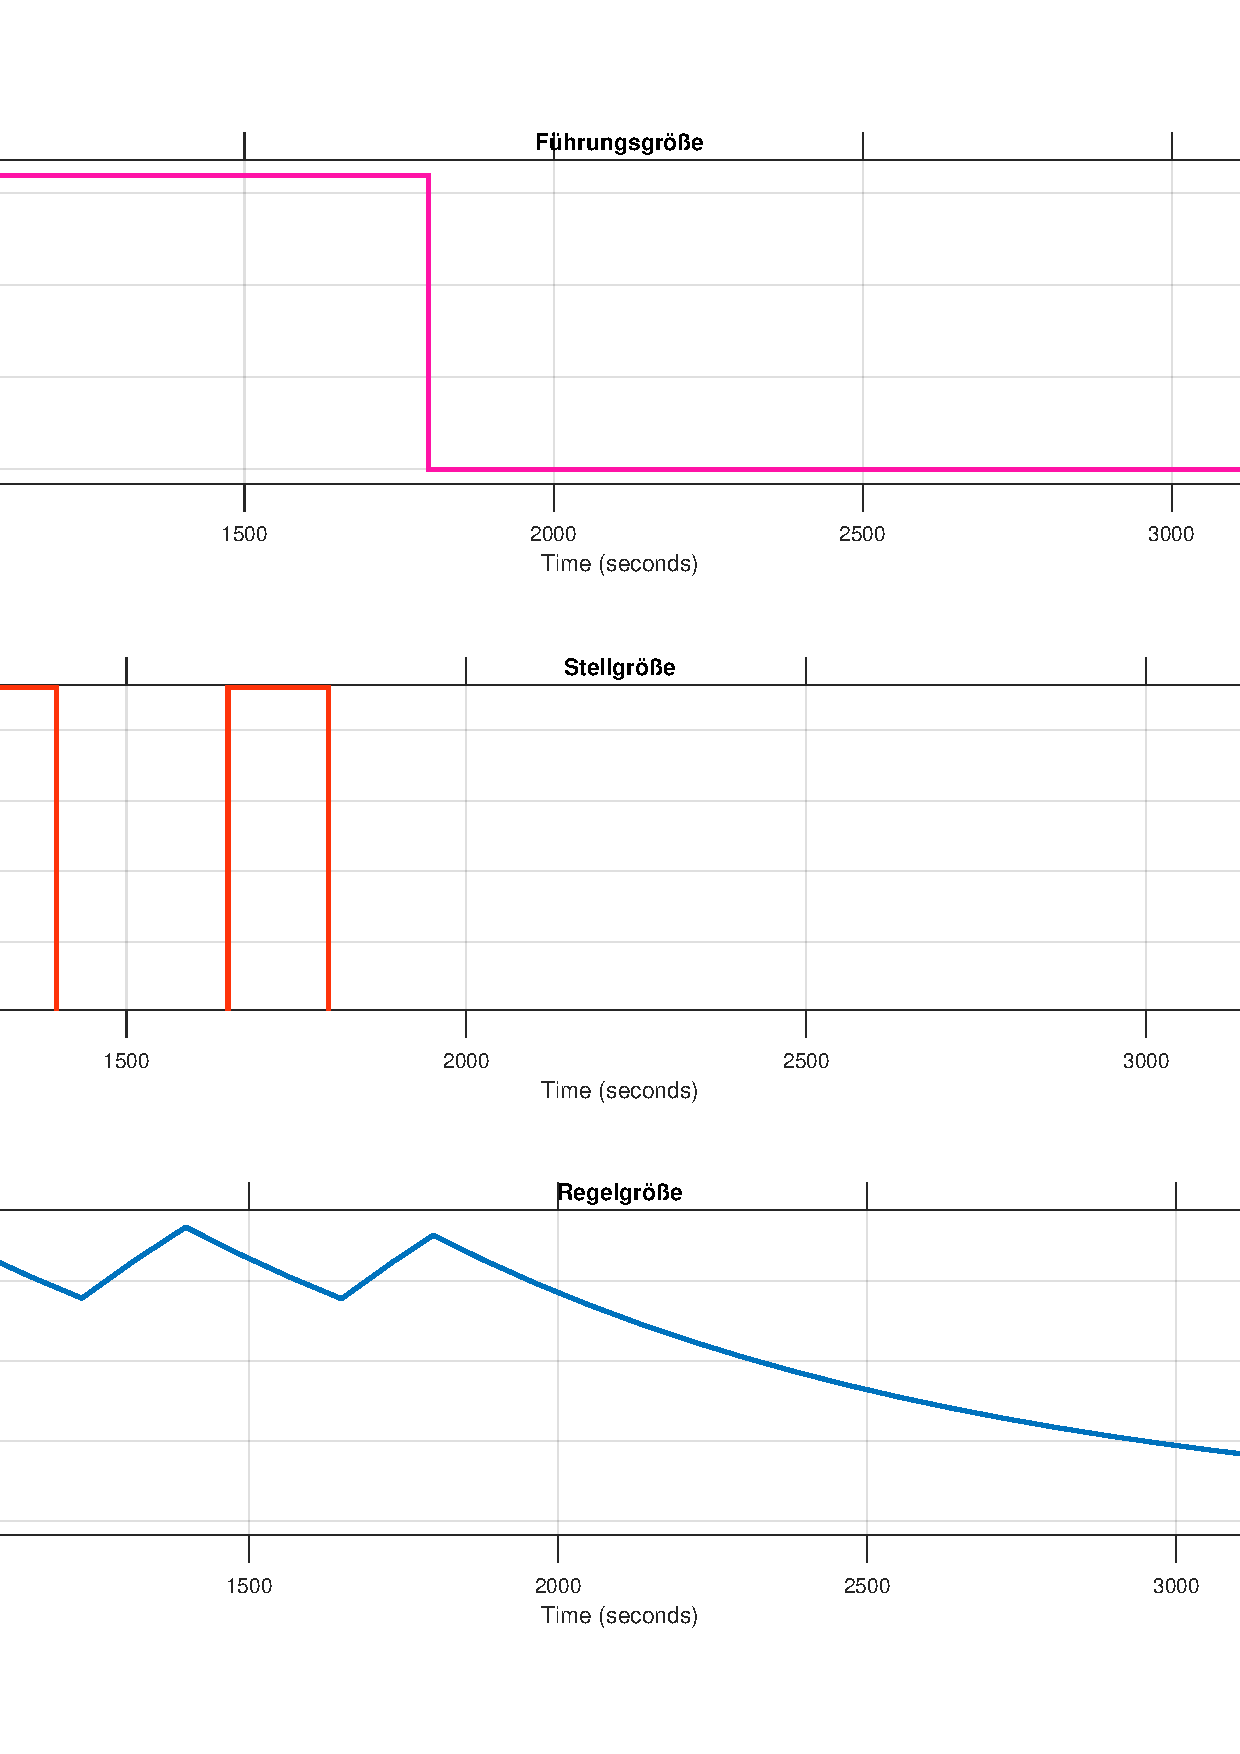
\includegraphics[width=\imagewidth]{../versuch1/temp_regler.pdf}
        \includesvg[width=\imagewidth, inkscapelatex=false]{../versuch1/temp_regler.svg}
        \caption{Zeitsignal der Regelgrößen}
        \label{fig:temp_regler}
    \end{figure*}

%-------------------------------------------------------------------------------------------------
%   Biblography
%-------------------------------------------------------------------------------------------------

\printbibliography[heading=bibnumbered]

\section{Autorenbeiträge}
    Maileen Schwenk und Jan Hoegen erstellten die Vorbereitung und Messauswertung. Jan Hoegen schrieb das Protokoll.

\section{Verfügbarkeit des Codes}
    Der Code zum Auswerten der Daten und Erstellen der Diagramme findet sich unter \url{https://github.com/JaxRaffnix/Regelungstechnik}. Ebenfalls ist hier der Code zum Erstellen dieser Ausarbeitung hinterlegt.

%-------------------------------------------------------------------------------------------------
%   Appendix
%-------------------------------------------------------------------------------------------------

\appendix

\section{MATLAB-Code der Sinussignale}
    \lstinputlisting[language=MATLAB, label={lst:sinus}]{../versuch1/sinus.m}

\section{MATLAB-Code zum Tiefpass}
    \lstinputlisting[language=MATLAB, label={lst:tiefpass}]{../versuch1/tiefpass.m}

\section{MATLAB-Code zum Temperaturregler}
    \lstinputlisting[language=MATLAB, label={lst:temp_regler}]{../versuch1/temp_regler_settings.m}

\end{document}